\section{Extending SyN for multi-modality images}

Let $I$, $J$ be two images defined over $\Omega_{I}$, $\Omega_{J}$, respectively. We consider $\Omega_{I}, \Omega_{J}$ as the transformed grids $\mathcal{L}_{I}$, $\mathcal{L}_{J}$
associated to $I, J$, under their corresponding grid-to-space transforms $\mathcal{A}_{I}$, $\mathcal{A}_{J}$ (fig. \ref{fig:syn_overview}). Let $G$ be the set of possible intensity
values these images may take (e.g. $G=\left\lbrace 0,1,...,255\right\rbrace$). We aim to find two diffeomorphisms
$\phi_{I}:\Omega_{I}\rightarrow \Omega_{R}$, $\phi_{J}:\Omega_{J}\rightarrow \Omega_{R}$ such that the images get aligned in the reference space $\Omega_{R}$
after warping them under $\phi_{I}^{-1}$ and $\phi_{J}^{-1}$. In other words, for each point $x \in \Omega_{R}$, $I(\phi_{I}^{-1}(x))$ is mapped to $J(\phi_{J}^{-1}(x))$
(fig. \ref{fig:syn_overview}). To handle multi-modality images, we will model the intensity correspondence between the two images using two conditionally independent transfer functions.
More precisely:
\begin{equation}\label{eq:SyNEM_gom_ref}
    \begin{array}{ccccc}
        F_{J}\left[J(\phi_{J}^{-1}(x))\right] &=& I(\phi_{I}^{-1}(x)) &+& \eta_{J}(x)\\
        F_{I}\left[I(\phi_{I}^{-1}(x))\right] &=& J(\phi_{J}^{-1}(x)) &+& \eta_{I}(x)
    \end{array}, x\in\Omega_{R},
\end{equation}
where $\eta_{I}, \eta_{J}$ are random fields. In general, we cannot assume independence between $\eta_{I}$ and $\eta_{J}$ because there is some unknown relationship between $I$ and $J$.
Instead, we assume conditional independence: given $F_{J}[J(\phi_{J}^{-1}(\cdot))]$, the random field $\eta_{J}$ is independent from $\eta_{I}$. Analogously, given
$F_{I}[I(\phi_{I}^{-1}(\cdot))]$, the random field $\eta_{I}$ is independent from $\eta_{J}$. In addition, we assume independence within each random field, i.e.
\hbox{$\eta_{I}(x) \perp \eta_{I}(y)$} and \hbox{$\eta_{J}(x) \perp \eta_{J}(y)$} \hbox{$\forall x,y\in\Omega_{R}$}. This formulation differs from Arce {\it et al.} \cite{Arce-santana2014} in that
we are taking advantage of both modalities by estimating transfer functions in both directions. Notice that, by assuming the random variables
$\eta_{I}(x), \eta_{J}(x), x\in\Omega_{R}$ are normally distributed, Arce {\it et al.} \cite{Arce-santana2014} are implicitly assuming that there is a functional dependency
between the two modalities, which in general is not true. However, similar studies, most notably Roche et al. \cite{Roche1998} have found that in brain image registration of several
modalities, the assumption of a functional dependency is not critical.
%the transfer function is surjective
%(in other words, there is a functional dependency between the two modalities),
%which, in general, is not true. Although this condition may seem too strong, the same formulation implicitly introduces a mechanism to alleviate the effect of having non-surjective
%transfer functions: if an intensity value $g\in G$ in the first modality maps to multiple intensities, say $h_{1}, ..., h_{k}\in G$, in the second modality, the estimated variance
%will be large, which will reduce the contribution of all those voxels having intensity $g$. By considering both transfer functions instead of arbitrarily choosing one of them, we
%are not solving the issue of non-surjective transfers, since some intensities $h_{1}, ..., h_{k}$ may map more intensities, in addition to $g$, in the first modality (e.g. if the
%first transfer is not injective), but it may be the case that some of them only map to $g$, which will then be exploited by the algorithm since their estimated variance will be small,
%thus making their contribution stronger. In their experiments, Roche et al.\cite{Roche1998} found that in brain image registration of several modalities, the assumption of a functional dependency is not
%critical.\\

\begin{figure}[H]
\centering
\fbox{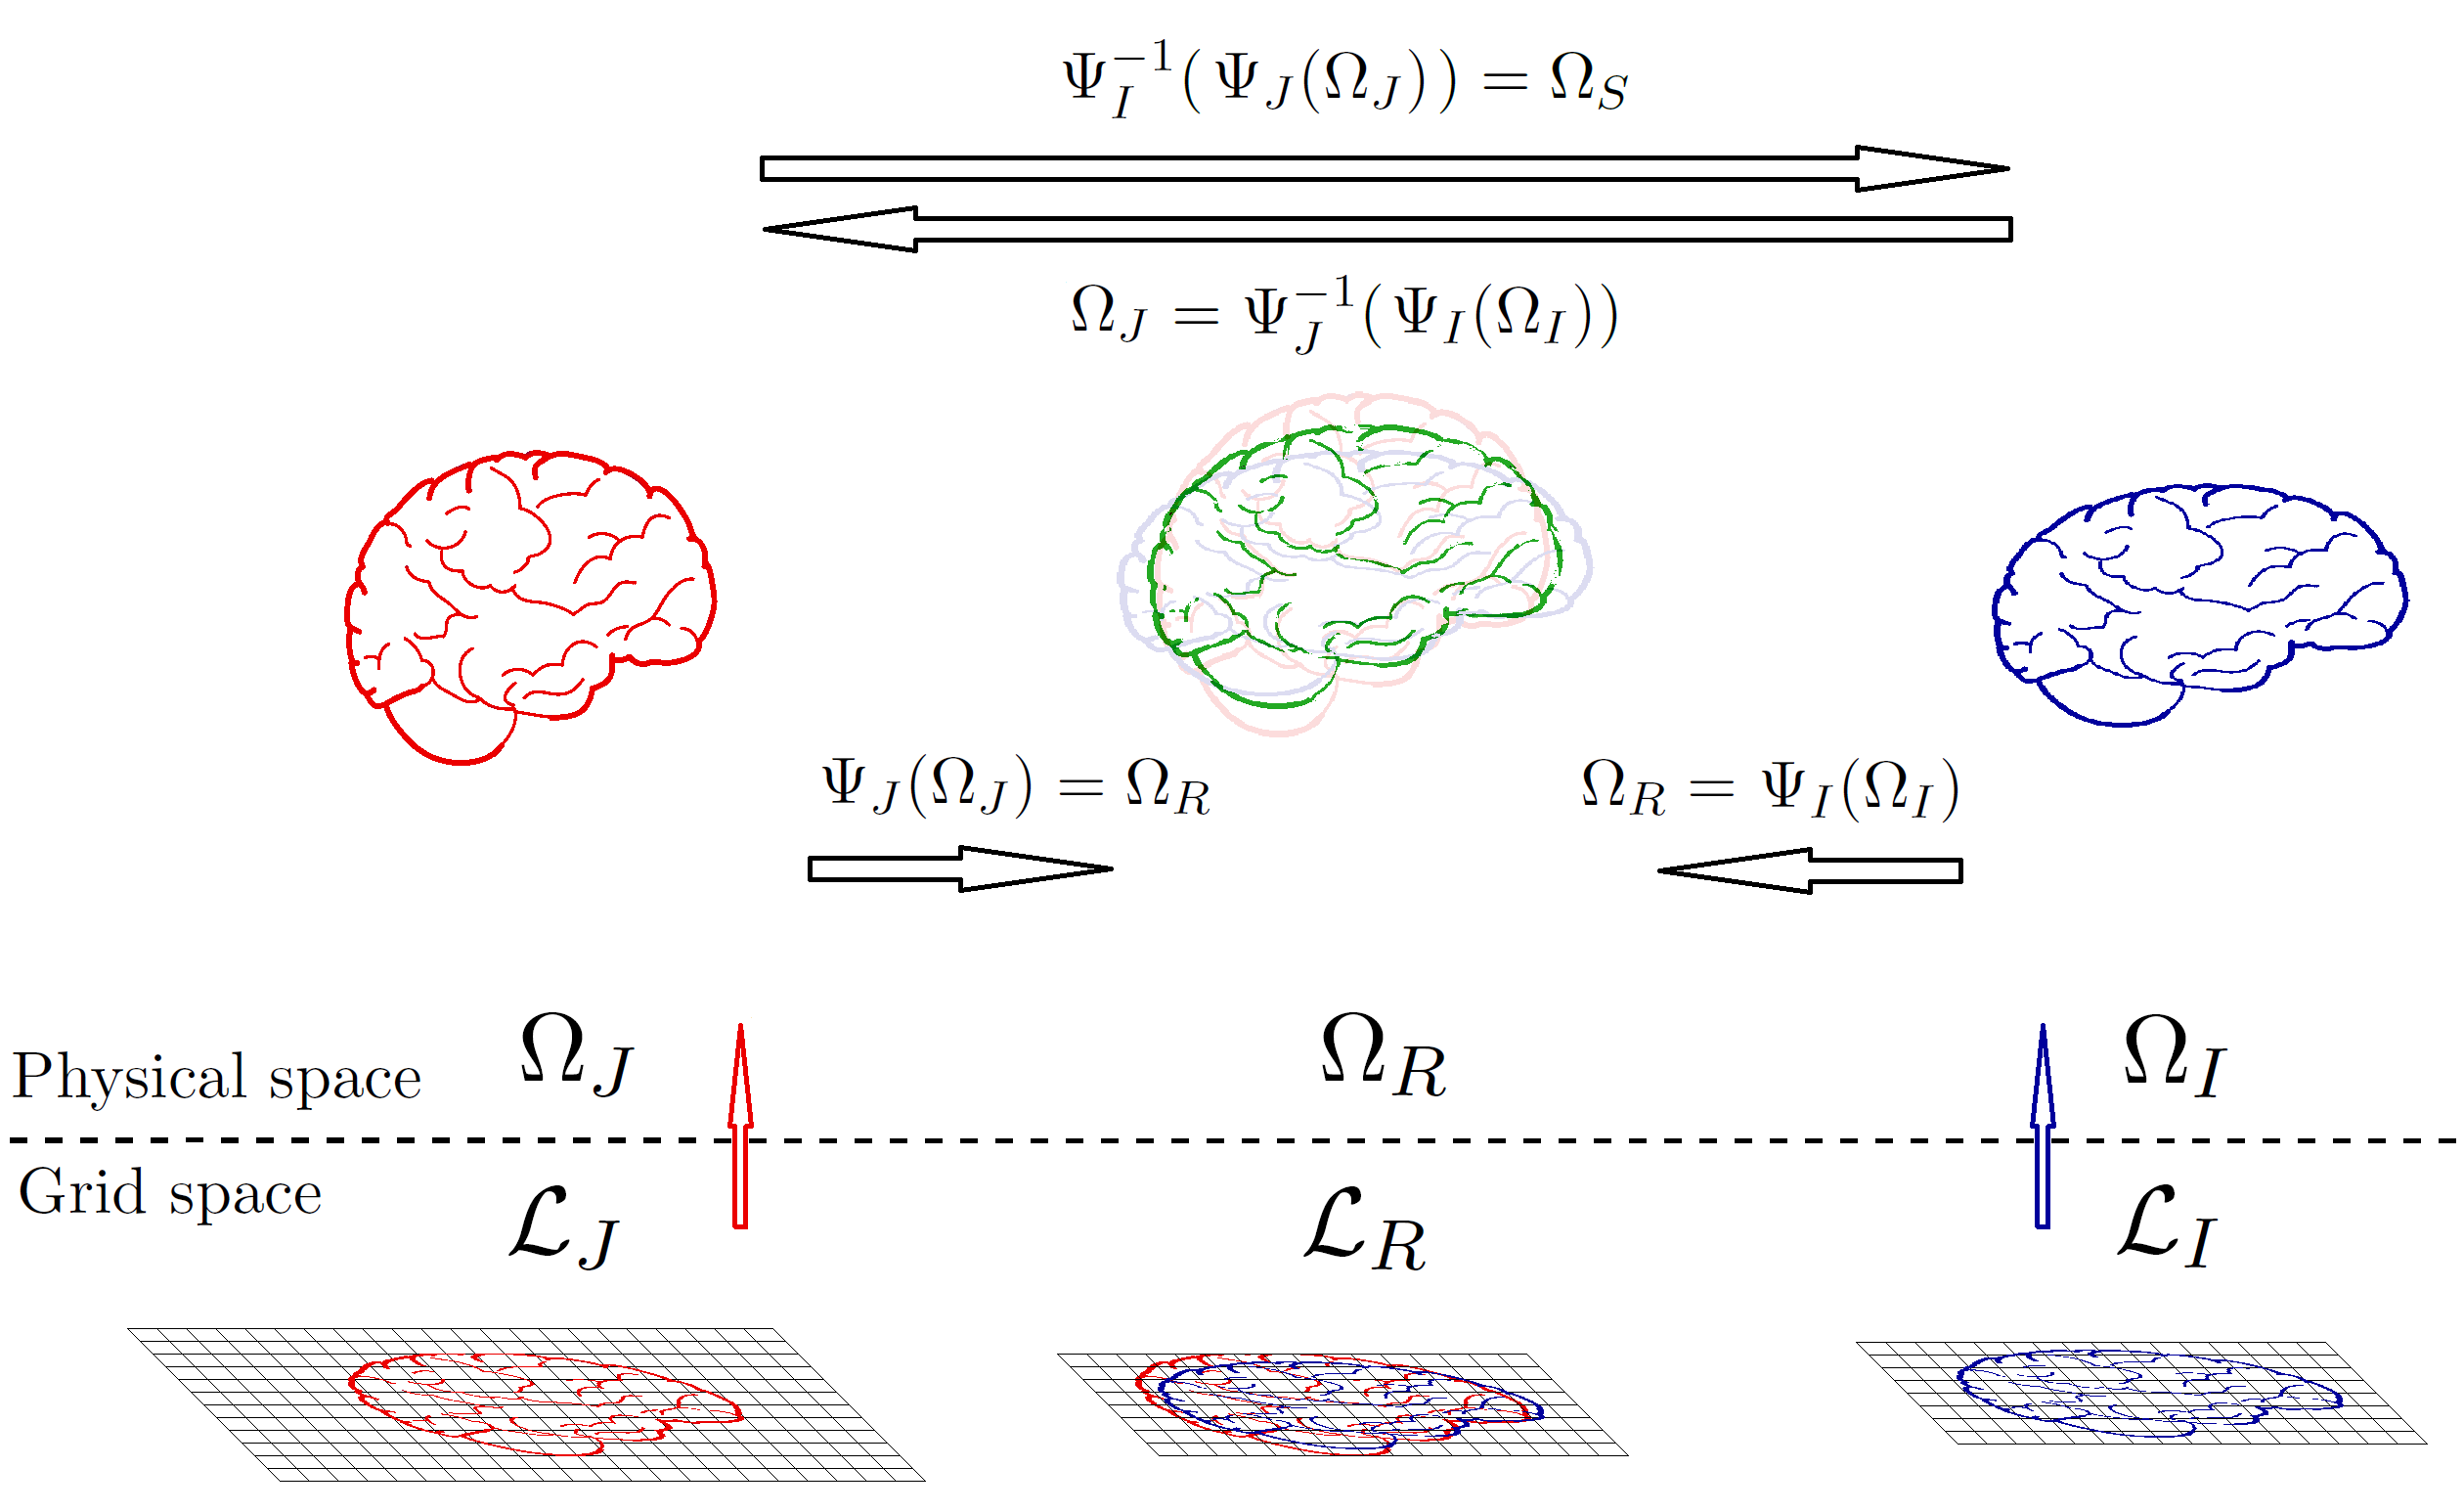
\includegraphics[width=1.0\linewidth]{./images/syn_overview.png}}
\caption{The Greedy SyN algorithm registers two input images by computing two diffeomorphisms that map the input images towards a common reference domain. The final
diffeomorphism is computed by composing the two partial diffeomorphisms.}
\label{fig:syn_overview}
\end{figure}

By defining the warped images \hbox{$\tilde{I}(x) = I(\phi_{I}^{-1}(x))$} and \hbox{$\tilde{J}(x) = J(\phi_{J}^{-1}(x))$} and the hidden random variables
\hbox{$Y(x) = F_{J}\left[\tilde{J}(x)\right]$}, \hbox{$Z(x) = F_{I}\left[\tilde{I}(x)\right]$, $x\in\Omega_{R}$}, our observation model can be written as
\begin{equation}\label{eq:SyNEM_gom_update}
    \begin{array}{ccccc}
    	Y(x) &=& \tilde{I}(x) &+& \eta_{J}(x)\\
        Z(x) &=& \tilde{J}(x) &+& \eta_{I}(x)
    \end{array}, x\in\Omega_{R}.
\end{equation}

These are precisely two instances of Arce's formulation (eq. 1 of \cite{Arce-santana2014}) in the reference space, and the conditional independence of $\eta_{I}, \eta_{J}$
given $Y, Z, \phi_{I}, \phi_{J}$ is made explicit. By performing similar computations as in \cite{Arce-santana2014} we can obtain the EM cost function as:
\begin{equation}\label{eq:SyNEM_energy}
    Q(\phi_{I}, \phi_{J}) = \sum_{x \in \Omega_{R}} \frac{\left(\overline{Y}(x) - \tilde{I}(x)\right)^{2}}{2\sigma^{2}_{Y}(x)} +
                                                     \frac{\left(\overline{Z}(x) - \tilde{J}(x)\right)^{2}}{2\sigma^{2}_{Z}(x)} dV +
                                                     \lambda\left(R(\phi_{I}) + R(\phi_{J})\right),
\end{equation}
where $\phi_{I}^{(0)}, \phi_{J}^{(0)}$ are initial approximations of the transformations, and
\begin{equation}
    \begin{array}{lll}
        \overline{Y} &=& E\left[\left.Y \right| I, J, \phi_{I}^{(0)}, \phi_{J}^{(0)}\right]\\
        \overline{Z} &=& E\left[\left.Z \right| I, J, \phi_{I}^{(0)}, \phi_{J}^{(0)}\right]\\
        \sigma_{Y}^{2}(x) &=& Var\left[\left.Y(x) \right| I, J, \phi_{I}^{(0)}, \phi_{J}^{(0)}\right]\\
        \sigma_{Z}^{2}(x) &=& Var\left[\left.Z(z) \right| I, J, \phi_{I}^{(0)}, \phi_{J}^{(0)}\right]
    \end{array}
\end{equation}

Notice that Arce's metric \cite{Arce-santana2014}, may be regarded as a generalization of the Correlation Ratio proposed by
Roche et al. \cite{Roche1998}: if we assume $\sigma^{2}_{Z}(x) = \sigma^{2}_{Z}$ (constant for all $x\in\Omega_{R}$) then, according to
eq.(\ref{eq:SyNEM_gom_update}),\hbox{$\left[Z(x) - \tilde{J}(x)\right] \sim N(0, \sigma^{2}_{Z})$}, and
\begin{equation}
    \frac{1}{|\Omega_{R}|}\sum_{x \in \Omega_{R}} \frac{\left(\overline{Z}(x) - \tilde{J}(x)\right)^{2}}{\sigma^{2}_{Z}(x)} =
    \frac{Var\left[Z - \tilde{J}\right]}{Var\left[Z\right]},
\end{equation}
the Correlation Ratio. Here, we have written simply $Var[\cdot]$ to denote the conditional sample variance given $ I, J, \phi_{I}^{(0)}, \phi_{J}^{(0)}$.\\

Equation \ref{eq:SyNEM_energy} can be efficiently minimized by following Vercauteren's analysis of the \textit{diffeomorphic demons} algorithm \cite{Vercauteren2009} as follows. Let's choose the regularization function $R(\cdot) = ||\nabla \cdot||^{2}$. Given
an initial approximation of $\phi_{J}^{-1}$, we wish to find a small update displacement field $\mathbf{u}$, which minimizes:
\begin{equation}\label{eq:vercauteren_cost}
    Q(\mathbf{u}) = \sum_{x \in \Omega_{R}} \frac{\left(\overline{Z}(x) - \tilde{J}(x + \mathbf{u}(x))\right)^{2}}{\sigma^{2}_{Z}(x)} + \lambda ||\nabla \mathbf{u}||^{2}.
\end{equation}

Minimizing this energy can be accomplished by introducing an auxiliary deformation field $\mathbf{v}$ and a modified energy function
\begin{equation}\label{eq:vercauteren_extended_cost}
    Q(\mathbf{u}, \mathbf{v}) = \sum_{x \in \Omega_{R}} \frac{(\overline{Z}(x) - \tilde{J}(x + \mathbf{u}(x)))^{2}}{\sigma^{2}_{Z}(x)} dV + \frac{1}{\tau}||\mathbf{u}-\mathbf{v}||^{2}+\lambda ||\nabla \mathbf{v}||^{2},
\end{equation}
the optimization can then be accomplished by alternating two steps. In the first step we optimize with respect to $\mathbf{u}$ starting with $\mathbf{v} = 0$
\begin{equation}\label{eq:vercauteren_step1}
    \widehat{\mathbf{u}} = \arg\min_{\mathbf{u}}\sum_{x \in \Omega_{R}} \frac{(\overline{Z}(x) - \tilde{J}(x+\mathbf{u}(x)))^{2}}{\sigma^{2}_{Z}(x)} dV + \frac{1}{\tau} ||\mathbf{u}||^{2}.
\end{equation}
We can perform a point-wise minimization by using the first order approximation around the identity
$\tilde{J}(x+\mathbf{u}(x)) \approx \tilde{J}(x) + \nabla \tilde{J}(x)^{T}\mathbf{u}(x)$ and then equating to zero the derivative with respect to $\mathbf{u}(x)$ to obtain:
\begin{equation}\label{eq:euler_lagrange_step1}
    \widehat{\mathbf{u}}(x) = \frac{\overline{Z}(x) - \tilde{J}(x)}{||\nabla \tilde{J}(x)||^{2} + \frac{\sigma_{Z}^{2}(x)}{\tau}}\nabla \tilde{J}(x).
\end{equation}
This expression corresponds to equation 4 in Vercauteren {\it et al.} \cite{Vercauteren2009}, but in their work, the factor $\sigma_{Z}^{2}(x)$
is approximated by $\sigma_{Z}(x) \approx |\overline{Z}(x) - \tilde{J}(x)|$ to obtain the traditional {\it demons} step. However, in our case as in Arce
{\it et al.}\cite{Arce-santana2014}, we have an explicit and natural estimation of $\sigma^{2}_{Z}(x)$.\\

The second step minimizes eq. \ref{eq:vercauteren_extended_cost} with respect to $\mathbf{v}$ and with $\mathbf{u}=\widehat{\mathbf{u}}$ previously obtained. It can be
shown that the solution of this second sub-problem is the convolution of $\widehat{\mathbf{u}}$ with a Gaussian kernel\cite{Vercauteren2009}.\\
%To update diffeomorphisms $\phi_{I}, \phi_{J}$ we need to take into consideration that we used their inverses to map images $I, J$ to the reference space. A direct expansion of
%$\tilde{I} \circ \psi$ yields $\phi_{I}^{-1} \leftarrow \phi_{I}^{-1} \circ \psi$, taking its inverse yields $\phi_{I} \leftarrow \psi^{-1} \circ \phi_{I}$, where
%$\psi^{-1} = Id - \mathbf{u}$ for a small displacement field $\mathbf{u}$. We adopted this strategy rather than directly updating the inverses so that the resulting algorithm
%(alg. \ref{alg:SyNEM})is equivalent to the Greedy SyN algorithm previously described (alg. \ref{alg:Greedy_SyN}), which has been extensively tested by the neuroimaging
%community.

\begin{algorithm}[h!]
\caption{SyN-EM}\label{alg:SyNEM}
\begin{algorithmic}[1]
\STATE Initialize: $\phi_{I} = Id, \phi_{J} = Id$
\REPEAT
    \STATE Warp $\tilde{I}  = I \circ \phi_{I}^{-1}, \tilde{J} = J \circ \phi_{J}^{-1}$
    \STATE E-Step: $\bar{I} = E[F_{I}(\tilde{I})]$, $\bar{J} = E[F_{J}(\tilde{J})]$ given $\phi_{I}, \phi_{J}$
    \STATE Compute update for $\phi_{J}$: $\mathbf{u}_{I} = \frac{\bar{J}(x) - \tilde{I}(x)}{||\nabla \tilde{I}(x)||^{2} + \frac{\sigma_{J}^{2}(x)}{\tau}}\nabla \tilde{I}(x)$
    \STATE Compute update for $\phi_{I}$: $\mathbf{u}_{J} = \frac{\bar{I}(x) - \tilde{J}(x)}{||\nabla \tilde{J}(x)||^{2} + \frac{\sigma_{I}^{2}(x)}{\tau}}\nabla \tilde{J}(x)$
    \STATE Smooth $\mathbf{u}_{I} = K \ast \mathbf{u}_{I}$
    \STATE Smooth $\mathbf{u}_{J} = K \ast \mathbf{u}_{J}$
    \STATE Update $\phi_{I} = (Id - \mathbf{u}_{I}) \circ \phi_{I}$
    \STATE Update $\phi_{J} = (Id - \mathbf{u}_{J}) \circ \phi_{J}$
    \STATE Invert $\phi_{I}^{-1}, \phi_{J}^{-1} = invert(\phi_{I}), invert(\phi_{J})$
    \STATE Invert $\phi_{I}, \phi_{J} = invert(\phi_{I}^{-1}), invert(\phi_{J}^{-1})$
\UNTIL{Convergence}
\RETURN $\phi_{I}, \phi_{J}$
\end{algorithmic}
\end{algorithm}


\subsection{Expected Cross-Correlation}
The SyN-EM algorithm (alg. \ref{alg:SyNEM}) may be regarded as a counterpart of SSD for multi-modality images. The main drawback of using a point-wise metric like SSD is that
it is unable to capture important features from the voxels' neighborhoods like gradients and texture. This makes point-wise metrics more susceptible to noise and image artifacts
such as the bias field in MRI. By considering small windows around each voxel, the Cross Correlation metric takes advantage of this local information resulting in a more robust
metric.\\

The EM formulation belongs the class of multi-modal image registration methods that reduce the multi-modality problem to a mono-modality one\cite{Sotiras2013}. One of the
advantages of this class of methods is that it is relatively easy to extend them to other mono-modal metrics. In particular, we can extend the SyN-EM algorithm to consider
local neighborhoods by defining the {\it Expected Cross Correlation} metric as:

\begin{equation}\label{eq:ecc_metric}
    \Pi_{ECC}(\tilde{I}, \tilde{J} | \phi_{I}, \phi_{J}) = \frac{<\bar{I}, \tilde{J}>^{2}}{||\bar{I}||^{2}||\tilde{J}||^{2}} + \frac{<\tilde{I}, \bar{J}>^{2}}{||\tilde{I}||^{2}||\bar{J}||^{2}}
\end{equation}
where $\tilde{I} = I\circ \phi_{I}^{-1}$, $\tilde{J} = J\circ \phi_{J}^{-1}$, are the warped images to the reference space and
$\bar{I} = E[F_{I}[\tilde{I}]|\phi_{I}, \phi_{J}]$, $\bar{J} = E[F_{J}[\tilde{J}]|\phi_{I}, \phi_{J}]$. The first term corresponds to the CC metric, in reference space,
between $\tilde{J}$ and the expected value of $F_{I}[\tilde{I}]$ given $\phi_{I}, \phi_{J}$, which is the ``predicted'' image $\tilde{I}$ under the modality of $\tilde{J}$,
assuming the $\phi_{I}, \phi_{J}$ correctly align $I$ and $J$. The second term corresponds to the CC metric in the other modality. The resulting algorithm (\ref{alg:SyNECC})
is, therefore, a combination of the Greedy-SyN algorithm (\ref{alg:Greedy_SyN}) (computing the diffeomorphism updates) and the SyN-EM algorithm (updating our estimates
for $E[F_{I}[\tilde{I}]]$, $E[F_{J}[\tilde{I}]]$ given new estimated diffemorphisms $\phi_{I}, \phi_{J}$).

\begin{algorithm}[h!]
\caption{SyN-ECC}\label{alg:SyNECC}
\begin{algorithmic}[1]
\STATE Initialize: $\phi_{I} = Id, \phi_{J} = Id$
\REPEAT
    \STATE Warp $\tilde{I}  = I \circ \phi_{I}^{-1}, \tilde{J} = J \circ \phi_{J}^{-1}$
    \STATE E-Step: $\bar{I} = E[F_{I}(\tilde{I})]$, $\bar{J} = E[F_{J}(\tilde{J})]$ given $\phi_{I}, \phi_{J}$
    \STATE Compute the gradient $\nabla_{\phi_{I}} \Pi_{ECC}(\tilde{I}, \tilde{J} | \phi_{I}, \phi_{J})$
    \STATE Compute the gradient $\nabla_{\phi_{J}} \Pi_{ECC}(\tilde{I}, \tilde{J} | \phi_{I}, \phi_{J})$
    \STATE Update $\phi_{I}$ according to eq. \ref{eq:gsyn_update} using $\nabla_{\phi_{I}}$
    \STATE Update $\phi_{J}$ according to eq. \ref{eq:gsyn_update} using $\nabla_{\phi_{J}}$
    \STATE Invert $\phi_{I}^{-1}, \phi_{J}^{-1} = invert(\phi_{I}), invert(\phi_{J})$
    \STATE Invert $\phi_{I}, \phi_{J} = invert(\phi_{I}^{-1}), invert(\phi_{J}^{-1})$
\UNTIL{Convergence}
\RETURN $\phi_{I}, \phi_{J}$
\end{algorithmic}
\end{algorithm}
